\section{Optical Flow}
For each pixel in an image, optical flow determines the corresponding pixel in the next image: \cf{
    \text{Input: two frames}\quad\to\quad \text{Output: Optical flow field } (u,v)(x,y,t)
}
This can be cast as a \b{variational problem} and can be learned from rendered image parts.

\subsection{Horn-Schunck-Model}
The most basic model to start with is the Horn-Schunck-Model, which assumes two things:
\begin{enumerate}
    \item Gray value constancy (optic flow constraint):
    \cf{I(x+u, y+v, t+1)- I(x,y,t)=0 \quad\Leftrightarrow\quad I_xu+I_yu+I_t=0}
    \item Smoothness of the optic flow field:
    \f{
        \quad|\nabla u|^2 + |\nabla v|^2 \to \min
    }
\end{enumerate}
Combined in an energy function, this problem can be formalized as:
\cf{
    E(u,v) = \int_\Omega(I_xu+I_yu+I_t)^2 + \alpha(|\nabla u|^2 + |\nabla v|^2)dxdy
}

\subsection{Challenges for Optical Flow methods}
\b{6.2.1. Motion Discontinuities:\\[0.5em]}
Different, independently moving objects cause discontinuities in the correct flow field. The problem is that we usually do not know the object boundaries as not all edges are boundaries. This leads to the smoothness assumption not being satisfied everywhere.\\

\b{Problem:} With the quadratic smoothness penalizer we assume the assumption is satisfied everywhere, which leads to a Gaussian error distribution. \f{\to} Long deviations in tail of Guassian, drops fast to zero, too much influence given to outliers, leads to blurring. For this reason, we need to apply a robust error norm!\\

Applying a robust function \f{\Psi} (e.g. TV) to the smoothness term yields:
\cf{E_S(u,v)= \int_\Omega\Psi(|\nabla u|^2+|\nabla v|^2)dxdy}
This has the advantage that it is still convex with a global optimum but applies less penalty for larger deviations.\\
Minimizing the energy function \(E_S\) with Euler-Lagrange yields two divergence equations coupled by the diffusivity function \f{\Psi'}:
\cf{
    -\text{div}(\Psi'(|\nabla u|^2+|\nabla v|^2)\nabla u) = 0
}
\cf{
    -\text{div}(\Psi'(|\nabla u|^2+|\nabla v|^2)\nabla v) = 0
}
As the diffusivity depens on the unknown flow, this is a nonlinear system of equations.\\

To resolve the nonlinearity, one can apply the \b{lagged diffusivity / nonlinearity} scheme:
\begin{enumerate}
    \item Keep \f{\Psi'} fixed for an (initial) solution (u,v) (fixed point)
    \item Solve resulting linear system to obtain new fixed point
    \item Update \f{\Psi'} and iterate
\end{enumerate}
\vspace{0.5em}
\b{Left out: Discretization}
\newpage

\b{6.2.2. Occlusions:\\[0.5em]}
The problem with variational methods is that they only smooth the prior and thus match the pixels of the first image to the most similar pixel in the second image, even if they are now occluded and no matching would be possible.\\
This can be dealt with by applying a robust term (as before) to the \b{data term}:
\cf{E(u,v) = \int_\Omega\Psi\left((I_xu+I_yu+I_t)^2\right) + \alpha\Psi(|\nabla u|^2 + |\nabla v|^2)dxdy}
The resulting EL equations can be interpreted as giving less importance to pixels with high matching cost (i.e. occlusions). As this now results in a nonlinear term for the data too, we can again solve with lagged diffusivity.\\

\b{6.2.3. Illumination Changes:\\[0.5em]}
Illumination changes are typically caused by shadows, light source flickering, self-adaptive cameras, different viewing angles or non-Lambertian surfaces. These changes again lead to issues with the gray value constancy assumption.\\

To mitigate this issue, we introduce the \b{gradient} constancy assumption:
\cf{
    \nabla I(x+u, y+v, t+1) - \nabla I(x,y,t) = 0
}
Linearized this leads to second order derivatives and a new data term:
\cf{
    I_{xx}u+I_{xy}v+I_{xt}=0
}
\cf{
    I_{xy}u+I_{yy}v+I_{yt}=0
}
\cf{
    E_{GC} = \int_\Omega\Psi\left((I_{xx}u+I_{xy}v+I_{xt})^2+(I_{xy}u+I_{yy}v+I_{yt})^2\right)dxdy
}
Combining with the gray value assumption and the smoothness term leads to:
\cf{
    E(u,v) = \int_\Omega\Psi\left((I_xu+I_yu+I_t)^2\right)dxdy\\ + \gamma E_{GC} + \alpha E_S\quad ,
}
with separate robust penalizers \f{\Phi} for each feature, by which the best matching feature is automatically picked.\\

This has two important \b{positive effects}: More information by having two more equations AND invariance tp additive brightness changes.\\
\b{Negative effects} are: No rotation invariance AND more sensitivity to sensor noise. \\

\b{Note:} Using more descriptive features (Patches, CNNs) is possible but usually not advantageous:
\begin{itemize}
    \item Lower accuracy at motion discontinuities
    \item Descriptive power is mostly lost in the gradient
    \item Exploiting descriptive features for large displacement matching needs combinatorial optimization
\end{itemize}
\vspace{0.5em}
\b{6.2.4. Large Displacements:\\[0.5em]}
The linearized constancy assumptions assume that the image is a linear gradient. Locally (between two pixels) this is true, so the linearization is only valid for subpixel displacements. If the images are otherwise quite smooth (which they typically are not at all), this approximation is also good enough for larger displacements.\newpage

If we do not linearize, the energy functional results in:
\cf{
    E(u,v) = \int_\Omega\Psi\left((I(x+w)-I(x))^2\right)+\alpha\Psi(|\nabla u|^2+|\nabla v|^2)dx,\quad x:=(x,y,t); w:=(u,v,1)
}
Here, \f{w} is the optical flow vector. \f{w} can be any (initial) optical flow vector, used to compensate the image and for gradient calculation. This formula is now the correct description of the matching criterion (no approximation anymore), however there are two problem with this:
\begin{enumerate}
    \item Further source of nonlinearity in EL equations
    \item Not convex in \f{w} \f{\to} multiple local minima
\end{enumerate}
To solve this, we need the non-linearized constancy assumption, which with
\cf{
    I_x:=\delta_xI(x+w) \quad I_y:=\delta_yI(x+w) \quad I_z := I(x+w) - I(x)
}
results in a highly nonlinear system of EL equations (as unknowns are hidden in \f{I_z}). This would require another fixed point iteration loop. Note that \f{I_x,I_y} are the spatial derivatives of the motion compensated second image while \f{I_z} is the remaining difference between the first and second image.\\

\b{Motion Compensation:} The idea is to warp the second image by applying a known/guessed flow vector \f{w}. The second image at \f{(t+1)} is then calculated by:
\cf{
    \tilde{I}(x):=I(x+w) = I(x+u, y+v, t+1)
}
To get the next flow vector starting from the motion compensated image \f{\tilde{I}}, we can solve the nonlinear system using the Gauss-Newton method. The problem with this method still is that the non-linearized constancy constraint is not sufficient to get around the local minima.\\

\b{Continuation Method:} The continuation method solves the problem of finding the global minimum even though the energy function has many local minima. Through several smoothing levels, this method removes details (oscillations) from the image, wich also smoothes the energy.\\

From the smoothed image you get an optimum. This you can use as an initialization for the next less smoothed image, then find the optimum there and so on until you optimize original image/function.\\

A more efficient way to do this is by creating an \b{image pyramid} of more and more downsampled images (downsampling includes smoothing) and working on them.\\

\b{Summary of the numerical scheme:}
\begin{itemize}
    \item Two nested fixed point loops + linear solver
    \item Outer loop:
    \begin{itemize}
        \item Removes nonlinearity due to non-linearized constancy assumptions
        \item Leads to solving for an increment \f{(du^k,dv^k)} in each iteration
        \item Requires warping of the second input image
        \item Coupled with coarse-to-fine strategy
    \end{itemize}
    \item Inner loop:
    \begin{itemize}
        \item Removes the remaining nonlinearity in the increment \f{(du^k,dv^k)} due to nonquadratic penalizers
        \item Lagged nonlinearity: factors kept fixed in each iteration
    \end{itemize}
    \item Iterative solver for the remaining linear system
\end{itemize}

\newpage
\b{6.2.5. Really Large Displacements:\\[0.5em]}
The remaining problem with the continuation method is that it fails for fast motions of small (low-contrast) structures. This is because small structures get smoothed away at coarse levels of the pyramid, and if their independent motion is too fast to be estimated where they reappear, the continuation method ends up in the wrong minimum. This can be solved by \b{combinatorial methods}.\\

\b{Nearest neighbor matching:}
\begin{itemize}
    \item Simplest combinatorial method
    \item For each point in image 1 find the best matching point in image 2 (complexity: \f{O(N^2)} with naive approach, \f{O(N\log N)} with approximation)
    \item Requires unique features (Patches, HOG, SIFT) to match, otherwise mismatches (color usually not sufficient)
    \item No regularity constraint that avoids mismatches
\end{itemize}
\vspace{0.5em}
\b{Adding spatial constraints:} If a point A matches point B, then the corresponding neighbors should match too (the displacement vectors should be locally similar \f{\to} smoothness). This can be formulated as an Integer Quadratic Program (IQP), which is a NP-hard problem.\\

\b{Note:} 
\begin{itemize}
    \item Combinatorial methods with spatial constraints are NP hard, slow, and can only estimate integer displacements (usually pixel-accurate)
    \item For most matching problems we actually desire subpixelaccurate displacements (real-valued)
    \item Idea: Combine combinatorial and variational approach, where the combinatorial optimization yields large displacements and the variational optimization yields subpixel accuracy and computational efficiency \f{\to} Large displacement optical flow (LDOF)
\end{itemize}
\vspace{0.5em}
\b{LDOF:\\[0.5em]}
The combinatorial part of LDOF is simple nearest neighbor matching of HOG descriptors, while the variational part is the classical coarse-to-fine warping strategy.\\
\begin{figure}[h!]
    \centering
    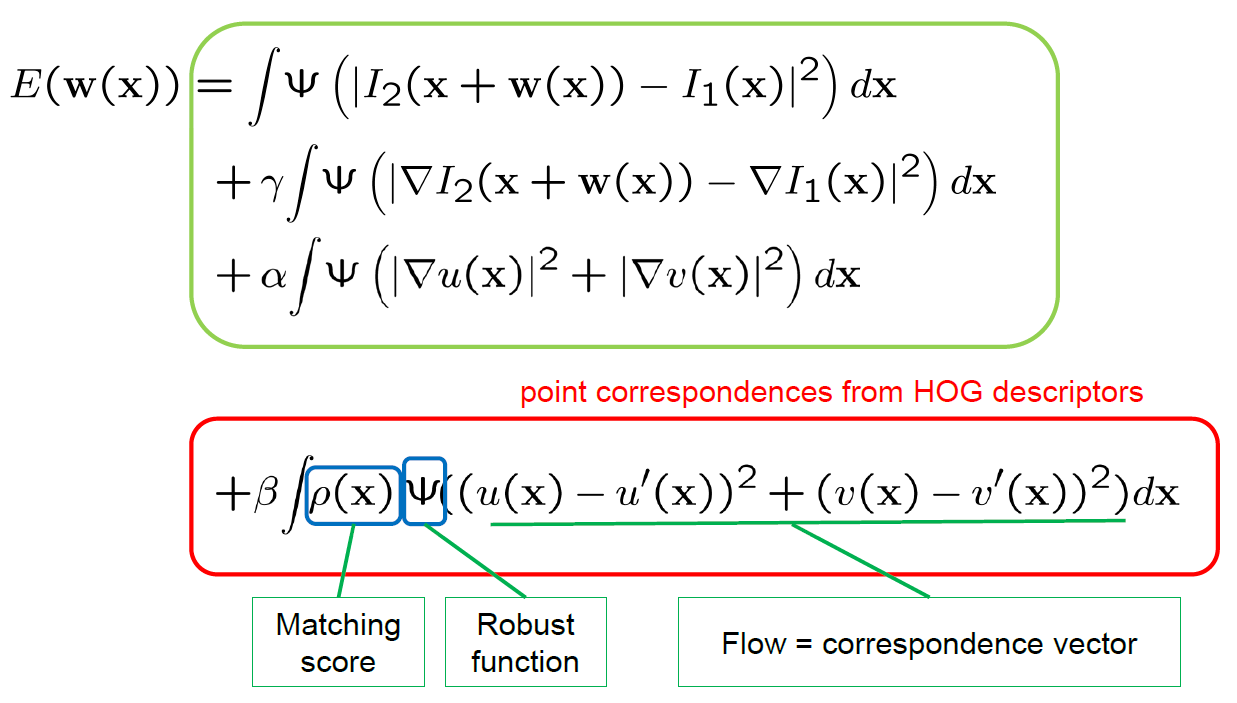
\includegraphics[width=0.6\textwidth]{flow.png}
\end{figure}

\b{Coarsed-to-fine effect:} At the beginning (low-res) you have a high number of nearest neighbor matches (computed at high-res) compared to the number of pixels. By improving the resolution the outlier matches are removed step-by-step.

\subsection{Optical Flow with a Deep Network}
\begin{itemize}
    \item Two images at input. Encoder who analyses that information
    \item Decoder produces optical flow field at the original resolution
    \item Problem: Where to get the data and ground truth optical flow field? \f{\to} Synthetic data
    \item \b{FlowNetC:} Two input CNNs learn features that are good to match. These features then get correlated in a special correlation layer, which produces a cost volume with the result of the correlation. The decoder can then analyze the cost volume and produce optical flow.
    \item \b{FlowNet2:} Improved data and training schedules, stacking of networks with motion comp.
    \item \b{FlowNet3:} Residual connections across networks
    \item \b{Advantage:} As accurate as best classical methods but much faster.
    \item \b{PWC-Net:}
    \begin{itemize}
        \item Start with downsampled images, compute energy minimization and get initial flowfield that you upsample for the next iteration.
        \item Take the next upsampling resolution and do the same and take the upsampled flow field as initial one for the energy      minimization.
        \item Repeat until you are at the original resolution and get the final resulting flow field.
    \end{itemize}
    \item \b{RAFT:}
    \begin{itemize}
        \item Multi-scale cost volume (robust matching at cost volume level)
        \item Context encoder (improves sharp boundaries)
        \item Recurrent architecture for refinement
    \end{itemize}
    \item \b{Note:} Generalization properties are much better than for recognition networks!
\end{itemize}

\newpage